\documentclass[aspectratio=169,10pt]{beamer}

\usepackage[utf8]{inputenc}
\usepackage[T1]{fontenc}
\usepackage{lmodern}
\usepackage{amsmath,amssymb}
\usepackage{booktabs,tabularx,array,adjustbox}
\usepackage{tikz,pgfplots}
\usepackage[most]{tcolorbox}
\usepackage{graphicx,xcolor,ragged2e}
\pgfplotsset{compat=1.18}
\usetikzlibrary{arrows.meta,positioning,calc,decorations.pathreplacing}

% ---------- Palette (template Pertemuan 2) ----------
\definecolor{DeepNavy}{HTML}{073B4C}
\definecolor{Teal}{HTML}{118AB2}
\definecolor{SoftBlue}{HTML}{E8F4FA}
\definecolor{Orange}{HTML}{F26B21}
\definecolor{SoftOrange}{HTML}{FFF0E6}
\definecolor{Mint}{HTML}{D9F2EC}
\definecolor{Purple}{HTML}{6A4C93}
\definecolor{SoftPurple}{HTML}{F2ECFA}
\definecolor{Gold}{HTML}{F7B801}
\definecolor{SoftGold}{HTML}{FFF7D6}
\definecolor{GrayText}{HTML}{4A5568}
\definecolor{LightLine}{HTML}{D9E2EC}

% ---------- Beamer (template Pertemuan 2) ----------
\setbeamertemplate{navigation symbols}{}
\setbeamercolor{normal text}{fg=DeepNavy,bg=white}
\setbeamercolor{frametitle}{fg=DeepNavy,bg=white}
\setbeamerfont{frametitle}{size=\Large,series=\bfseries}
\setbeamertemplate{frametitle}{%
  \vspace{0.25em}\insertframetitle\par
  \vspace{-0.25em}\tikz{\draw[Orange,line width=1.15pt] (0,0)--(1.15,0);}\vspace{-0.48em}
}
\setbeamertemplate{footline}{%
\leavevmode\hbox{%
\begin{beamercolorbox}[wd=.46\paperwidth,ht=2.2ex,dp=1ex,leftskip=1em]{}\scriptsize MA25-31017 Pemodelan Komputasi dan Analisis Numerik\end{beamercolorbox}%
\begin{beamercolorbox}[wd=.36\paperwidth,ht=2.2ex,dp=1ex,center]{}\scriptsize Program Studi Matematika ITERA\end{beamercolorbox}%
\begin{beamercolorbox}[wd=.18\paperwidth,ht=2.2ex,dp=1ex,rightskip=1em plus1fil]{}\scriptsize \insertframenumber/\inserttotalframenumber\end{beamercolorbox}}%
}

% ---------- Boxes (template Pertemuan 2) ----------
\tcbset{enhanced,boxrule=.7pt,arc=2mm,left=2mm,right=2mm,top=1mm,bottom=1mm,fonttitle=\bfseries,before skip=1pt,after skip=1pt}
\newtcolorbox{bluebox}[1][]{colback=SoftBlue,colframe=Teal,title=#1}
\newtcolorbox{orangebox}[1][]{colback=SoftOrange,colframe=Orange,title=#1}
\newtcolorbox{greenbox}[1][]{colback=Mint,colframe=DeepNavy!55!Teal,title=#1}
\newtcolorbox{purplebox}[1][]{colback=SoftPurple,colframe=Purple,title=#1}
\newtcolorbox{goldbox}[1][]{colback=SoftGold,colframe=Gold!80!black,title=#1}
\newcommand{\highlight}[1]{\textcolor{Orange}{\textbf{#1}}}
\newcommand{\smallgray}[1]{\textcolor{GrayText}{\scriptsize #1}}
\newcommand{\excel}[1]{\texttt{\detokenize{#1}}}

\begin{document}

% ============ 1. COVER ============
\begin{frame}[plain]
\begin{tikzpicture}[remember picture,overlay]
  \fill[SoftBlue] (current page.north west) rectangle ([xshift=.48\paperwidth]current page.south west);
  \fill[white] ([xshift=.48\paperwidth]current page.north west) rectangle (current page.south east);
\end{tikzpicture}
\vspace{0.60cm}
\begin{columns}[T,totalwidth=\textwidth]
\begin{column}{.44\textwidth}
{\fontsize{21}{24}\selectfont\bfseries Hampiran Turunan\\Numerik}\par
\vspace{0.12cm}
\tikz{\draw[Orange,line width=1.5pt] (0,0)--(1.9,0);}\par
\vspace{0.15cm}
{\large Beda hingga, Polinom Newton,\\dan Ekstrapolasi Richardson}\par
\vspace{0.40cm}
\small MA25-31017 \textbullet\ Pertemuan 5\par
\small Program Studi Matematika\par
\small Institut Teknologi Sumatera\par
\vspace{0.28cm}
\textbf{Dosen Pengampu}\par
Rifky Fauzi\par
Dear Michiko Mutiara Noor
\end{column}
\begin{column}{.52\textwidth}
\vspace{0.05cm}
\begin{tikzpicture}
\begin{axis}[width=\linewidth,height=.54\textheight,axis lines=middle,
  xmin=-.15,xmax=1.25,ymin=.1,ymax=1.35,grid=both,grid style={LightLine!55},
  xlabel={$x$},ylabel={$f(x)$},xtick={0,0.5,1},ytick=\empty,
  xticklabels={$x_i-h$,$x_i$,$x_i+h$},tick label style={font=\scriptsize},label style={font=\scriptsize}]
\addplot[domain=0:1.15,Teal,very thick,samples=120]{-0.1*x^4 -0.15*x^3 -0.5*x^2 -0.25*x +1.25};
\addplot[Orange,very thick] coordinates {(0,1.25) (.5,.925)};
\addplot[Purple,very thick,dashed] coordinates {(0,1.25) (1,.25)};
\addplot[only marks,mark=*,mark size=2pt,Orange] coordinates {(0,1.25) (.5,.925) (1,.25)};
\node[font=\scriptsize,Orange,anchor=south west] at (axis cs:.07,1.05) {beda mundur};
\node[font=\scriptsize,Purple,anchor=north east] at (axis cs:.94,.55) {beda pusat};
\end{axis}
\end{tikzpicture}
\par\vspace{-0.15cm}
\centering\smallgray{Turunan sebagai kemiringan: dari fungsi kontinu menjadi formula komputasi.}
\end{column}
\end{columns}
\end{frame}

% ============ 2. MOTIVASI ============
\begin{frame}{Mengapa turunan dihampiri?}
\scriptsize
\begin{columns}[T,totalwidth=\textwidth]
\begin{column}{.50\textwidth}
\begin{bluebox}[Turunan adalah laju perubahan]
Pada banyak masalah komputasi, kita tidak selalu memiliki bentuk turunan analitik yang nyaman.
Fungsi bisa muncul sebagai data tabel, hasil simulasi, atau ekspresi rumit.
\end{bluebox}
\begin{orangebox}[Ide numerik]
Gantikan turunan lokal dengan kemiringan garis yang dibentuk dari nilai fungsi di sekitar titik.
\[
 f'(x_i)\approx \frac{\Delta f}{\Delta x}.
\]
\end{orangebox}
\begin{greenbox}[Hal yang perlu dilihat]
Akurasi formula, ukuran langkah $h$, dan pola galat ketika $h$ diubah.
\end{greenbox}
\end{column}
\begin{column}{.46\textwidth}
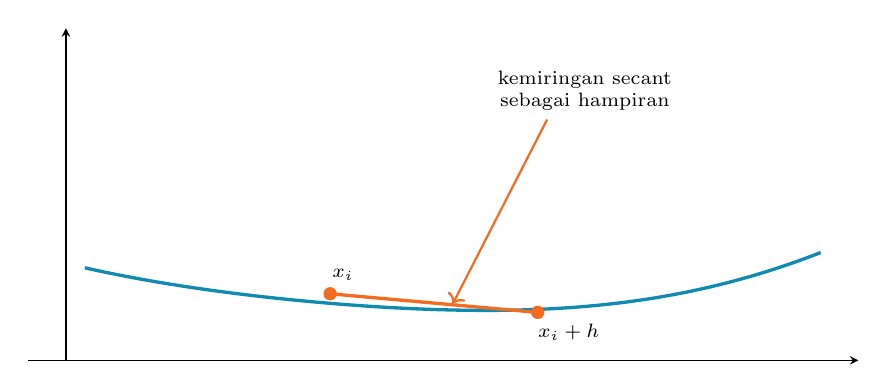
\begin{tikzpicture}
\begin{axis}[width=\linewidth,height=5.8cm,axis lines=middle,xmin=-.2,xmax=4.2,ymin=.2,ymax=4.2,xtick=\empty,ytick=\empty]
\addplot[domain=.1:4,Teal,very thick,samples=120]{.4 + .15*x + .20*(x-2.2)^2 + .15*sin(deg(1.2*x))};
\addplot[Orange,very thick] coordinates {(1.4,1.002) (2.5,0.778)};
\addplot[only marks,mark=*,mark size=2.2pt,Orange] coordinates {(1.4,1.002) (2.5,0.778)};
\node[font=\scriptsize,anchor=south west] at (axis cs:1.36,1.05) {$x_i$};
\node[font=\scriptsize,anchor=north west] at (axis cs:2.45,.75) {$x_i+h$};
\node[font=\scriptsize,align=center] at (axis cs:2.75,3.45) {kemiringan secant\\sebagai hampiran};
\draw[Orange,->,line width=.8pt] (axis cs:2.55,3.1)--(axis cs:2.05,.88);
\end{axis}
\end{tikzpicture}
\end{column}
\end{columns}
\end{frame}

% ============ 3. TAYLOR ============
\begin{frame}{Taylor sebagai mesin pembentuk rumus}
\scriptsize
\begin{columns}[T,totalwidth=\textwidth]
\begin{column}{.48\textwidth}
\begin{bluebox}[Ekspansi ke kanan]
\[
\begin{aligned}
f(x_i+h)=&\ f(x_i)+f'(x_i)h\\
&+\frac{f''(x_i)}{2!}h^2+\frac{f^{(3)}(x_i)}{3!}h^3\\
&+\frac{f^{(4)}(x_i)}{4!}h^4+\cdots
\end{aligned}
\]
\end{bluebox}
\end{column}
\begin{column}{.48\textwidth}
\begin{orangebox}[Ekspansi ke kiri]
\[
\begin{aligned}
f(x_i-h)=&\ f(x_i)-f'(x_i)h\\
&+\frac{f''(x_i)}{2!}h^2-\frac{f^{(3)}(x_i)}{3!}h^3\\
&+\frac{f^{(4)}(x_i)}{4!}h^4-\cdots
\end{aligned}
\]
\end{orangebox}
\end{column}
\end{columns}
\vspace{1mm}
\begin{greenbox}[Cara memperoleh formula]
Pilih kombinasi ekspansi Taylor, lalu isolasi turunan yang diinginkan. Suku yang tidak dipakai menjadi sumber galat pemotongan.
\end{greenbox}
\end{frame}

% ============ 4. THREE SCHEMES ============
\begin{frame}{Tiga skema turunan pertama}
\scriptsize
\begin{columns}[T,totalwidth=\textwidth]
\begin{column}{.32\textwidth}
\begin{bluebox}[Beda maju]
\[
f'(x_i)\approx \frac{f(x_i+h)-f(x_i)}{h}
\]
\centering
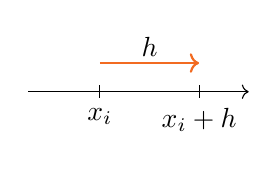
\begin{tikzpicture}[scale=.70]
\draw[->] (-.3,0)--(3.7,0);
\foreach \x/\lab in {1/$x_i$,2.8/$x_i+h$}{\draw (\x,.12)--(\x,-.12) node[below]{\lab};}
\draw[Orange,thick,->] (1,.52)--(2.8,.52);
\node at (1.9,.82){$h$};
\end{tikzpicture}
\end{bluebox}
\end{column}
\begin{column}{.32\textwidth}
\begin{orangebox}[Beda mundur]
\[
f'(x_i)\approx \frac{f(x_i)-f(x_i-h)}{h}
\]
\centering
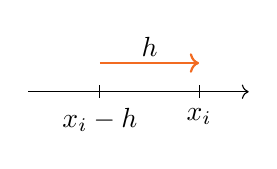
\begin{tikzpicture}[scale=.70]
\draw[->] (-.3,0)--(3.7,0);
\foreach \x/\lab in {1/$x_i-h$,2.8/$x_i$}{\draw (\x,.12)--(\x,-.12) node[below]{\lab};}
\draw[Orange,thick,->] (1,.52)--(2.8,.52);
\node at (1.9,.82){$h$};
\end{tikzpicture}
\end{orangebox}
\end{column}
\begin{column}{.32\textwidth}
\begin{purplebox}[Beda pusat]
\[
f'(x_i)\approx \frac{f(x_i+h)-f(x_i-h)}{2h}
\]
\centering
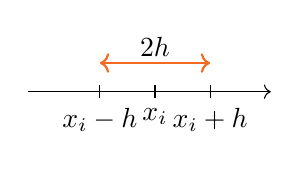
\begin{tikzpicture}[scale=.70]
\draw[->] (-.3,0)--(4.1,0);
\foreach \x/\lab in {1/$x_i-h$,2/$x_i$,3/$x_i+h$}{\draw (\x,.12)--(\x,-.12) node[below]{\lab};}
\draw[Orange,thick,<->] (1,.52)--(3,.52);
\node at (2,.82){$2h$};
\end{tikzpicture}
\end{purplebox}
\end{column}
\end{columns}
\vspace{1mm}
\begin{goldbox}[Bacaan geometri]
Beda maju melihat ke kanan, beda mundur melihat ke kiri, sedangkan beda pusat menyeimbangkan informasi dari kedua sisi.
\end{goldbox}
\end{frame}

% ============ 5 FORWARD DERIVATION ============
\begin{frame}{Beda maju: dari Taylor ke formula}
\scriptsize
\begin{columns}[T,totalwidth=\textwidth]
\begin{column}{.53\textwidth}
\begin{bluebox}[Mulai dari Taylor kanan]
\[
f(x_i+h)=f(x_i)+f'(x_i)h+\frac{f''(x_i)}{2}h^2+O(h^3).
\]
Pindahkan $f(x_i)$ dan bagi dengan $h$:
\[
\frac{f(x_i+h)-f(x_i)}{h}=f'(x_i)+\frac{f''(x_i)}{2}h+O(h^2).
\]
\end{bluebox}
\begin{orangebox}[Formula]
\[
f'(x_i)=\frac{f(x_i+h)-f(x_i)}{h}+O(h).
\]
\end{orangebox}
\end{column}
\begin{column}{.43\textwidth}
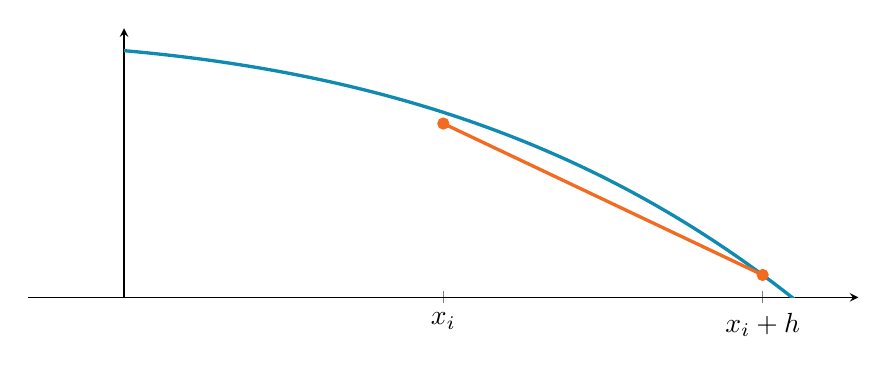
\begin{tikzpicture}
\begin{axis}[width=\linewidth,height=5.0cm,axis lines=middle,xmin=-.15,xmax=1.15,ymin=.15,ymax=1.35,xtick={.5,1},xticklabels={$x_i$,$x_i+h$},ytick=\empty]
\addplot[domain=0:1.08,Teal,very thick,samples=120]{-0.1*x^4 -0.15*x^3 -0.5*x^2 -0.25*x +1.25};
\addplot[Orange,very thick] coordinates {(.5,.925) (1,.25)};
\addplot[only marks,mark=*,Orange] coordinates {(.5,.925) (1,.25)};
\end{axis}
\end{tikzpicture}
\smallgray{Formula memakai dua titik: $x_i$ dan $x_i+h$.}
\end{column}
\end{columns}
\end{frame}

% ============ 6 BACKWARD CENTRAL ============
\begin{frame}{Beda mundur dan beda pusat}
\scriptsize
\begin{columns}[T,totalwidth=\textwidth]
\begin{column}{.48\textwidth}
\begin{orangebox}[Beda mundur]
Dari Taylor kiri:
\[
f(x_i-h)=f(x_i)-f'(x_i)h+\frac{f''(x_i)}{2}h^2+O(h^3).
\]
Maka
\[
f'(x_i)=\frac{f(x_i)-f(x_i-h)}{h}+O(h).
\]
\end{orangebox}
\end{column}
\begin{column}{.48\textwidth}
\begin{purplebox}[Beda pusat]
Kurangkan Taylor kiri dari Taylor kanan:
\[
f(x_i+h)-f(x_i-h)=2hf'(x_i)+\frac{2h^3}{3!}f^{(3)}(x_i)+O(h^5).
\]
Maka
\[
f'(x_i)=\frac{f(x_i+h)-f(x_i-h)}{2h}+O(h^2).
\]
\end{purplebox}
\end{column}
\end{columns}
\vspace{1mm}
\begin{greenbox}[Kesimpulan]
Beda pusat memiliki orde galat lebih tinggi karena suku-suku genap pada Taylor saling menghilangkan.
\end{greenbox}
\end{frame}

% ============ 7 VISUAL ============
\begin{frame}{Visualisasi skema beda hingga}
\scriptsize
\centering
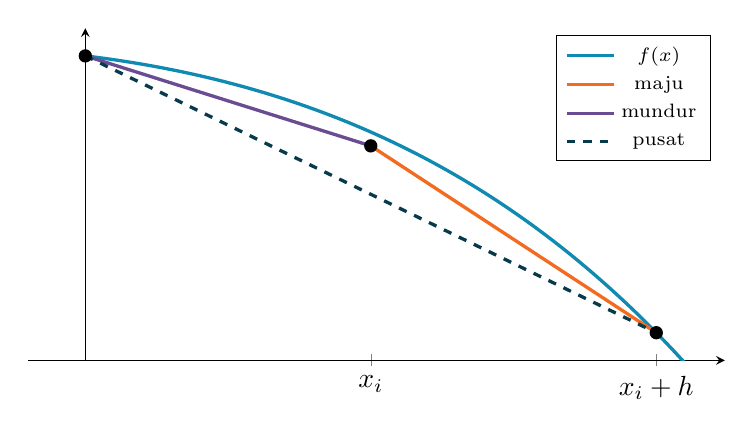
\begin{tikzpicture}
\begin{axis}[width=.86\linewidth,height=5.8cm,axis lines=middle,xmin=-.1,xmax=1.12,ymin=.15,ymax=1.35,xtick={0,.5,1},xticklabels={$x_i-h$,$x_i$,$x_i+h$},ytick=\empty,legend style={at={(0.98,0.98)},anchor=north east,font=\scriptsize}]
\addplot[domain=0:1.08,Teal,very thick,samples=160]{-0.1*x^4 -0.15*x^3 -0.5*x^2 -0.25*x +1.25};
\addlegendentry{$f(x)$}
\addplot[Orange,very thick] coordinates {(.5,.925) (1,.25)};
\addlegendentry{maju}
\addplot[Purple,very thick] coordinates {(0,1.25) (.5,.925)};
\addlegendentry{mundur}
\addplot[DeepNavy,very thick,dashed] coordinates {(0,1.25) (1,.25)};
\addlegendentry{pusat}
\addplot[only marks,mark=*,mark size=2.2pt] coordinates {(0,1.25) (.5,.925) (1,.25)};
\end{axis}
\end{tikzpicture}
\vspace{-1mm}
\begin{goldbox}[Pertanyaan kelas]
Jika titik yang digunakan berbeda, apakah galatnya harus sama? Apa yang terjadi ketika $h$ diperkecil?
\end{goldbox}
\end{frame}

% ============ 8 WORKED EXAMPLE ============
\begin{frame}{Contoh hitung: bandingkan $h=0.5$ dan $h=0.25$}
\scriptsize
\begin{bluebox}[Fungsi uji]
\[
f(x)=-0.1x^4-0.15x^3-0.5x^2-0.25x+1.25,
\quad x_i=0.5.
\]
\[
f'(x)=-0.4x^3-0.45x^2-x-0.25,
\quad f'(0.5)=-0.9125.
\]
\end{bluebox}
\begin{columns}[T,totalwidth=\textwidth]
\begin{column}{.49\textwidth}
\begin{orangebox}[h = 0.5]
\begin{tabular}{lcc}
\toprule
Skema & Hampiran & Galat relatif\\
\midrule
Maju & $-1.3500$ & $47.95\%$\\
Mundur & $-0.6500$ & $28.77\%$\\
Pusat & $-1.0000$ & $9.59\%$\\
\bottomrule
\end{tabular}
\end{orangebox}
\end{column}
\begin{column}{.49\textwidth}
\begin{greenbox}[h = 0.25]
\begin{tabular}{lcc}
\toprule
Skema & Hampiran & Galat relatif\\
\midrule
Maju & $-1.1547$ & $26.54\%$\\
Mundur & $-0.7141$ & $21.75\%$\\
Pusat & $-0.9344$ & $2.40\%$\\
\bottomrule
\end{tabular}
\end{greenbox}
\end{column}
\end{columns}
\vspace{1mm}
\smallgray{Nilai galat relatif dihitung terhadap $|f'(0.5)|$.}
\end{frame}

% ============ 9 SECOND DERIVATIVE ============
\begin{frame}{Turunan orde dua: petunjuk dari Taylor}
\scriptsize
\begin{columns}[T,totalwidth=\textwidth]
\begin{column}{.50\textwidth}
\begin{bluebox}[Pusatkan di $x_i$]
\[
\begin{aligned}
f(x_i+h)&=f_i+f_i'h+\frac{f_i''}{2}h^2+\frac{f_i^{(3)}}{6}h^3+\cdots,\\
f(x_i-h)&=f_i-f_i'h+\frac{f_i''}{2}h^2-\frac{f_i^{(3)}}{6}h^3+\cdots.
\end{aligned}
\]
Jumlahkan kedua persamaan:
\[
f(x_i+h)+f(x_i-h)=2f_i+f_i''h^2+O(h^4).
\]
\end{bluebox}
\end{column}
\begin{column}{.46\textwidth}
\begin{orangebox}[Formula pusat orde dua]
\[
f''(x_i)\approx
\frac{f(x_i+h)-2f(x_i)+f(x_i-h)}{h^2},
\]
\[
\text{galat }O(h^2).
\]
\end{orangebox}
\begin{greenbox}[Makna]
Turunan kedua melihat 	extbf{kelengkungan}: nilai tengah dibandingkan dengan rata-rata dua tetangganya.
\end{greenbox}
\end{column}
\end{columns}
\end{frame}

% ============ 10 SECOND DERIV OTHER ============
\begin{frame}{Turunan orde dua: maju, mundur, pusat}
\scriptsize
\begin{columns}[T,totalwidth=\textwidth]
\begin{column}{.32\textwidth}
\begin{bluebox}[Maju]
\[
f''(x_i)\approx\frac{f_i-2f_{i+1}+f_{i+2}}{h^2}
\]
\[
O(h)
\]
\centering
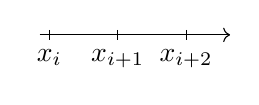
\begin{tikzpicture}[scale=.62]
\draw[->] (-.2,0)--(3.7,0);
\foreach \x/\lab in {0/$x_i$,1.4/$x_{i+1}$,2.8/$x_{i+2}$}{\draw (\x,.1)--(\x,-.1) node[below]{\lab};}
\end{tikzpicture}
\end{bluebox}
\end{column}
\begin{column}{.32\textwidth}
\begin{orangebox}[Mundur]
\[
f''(x_i)\approx\frac{f_i-2f_{i-1}+f_{i-2}}{h^2}
\]
\[
O(h)
\]
\centering
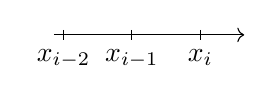
\begin{tikzpicture}[scale=.62]
\draw[->] (-.2,0)--(3.7,0);
\foreach \x/\lab in {0/$x_{i-2}$,1.4/$x_{i-1}$,2.8/$x_i$}{\draw (\x,.1)--(\x,-.1) node[below]{\lab};}
\end{tikzpicture}
\end{orangebox}
\end{column}
\begin{column}{.32\textwidth}
\begin{purplebox}[Pusat]
\[
f''(x_i)\approx\frac{f_{i+1}-2f_i+f_{i-1}}{h^2}
\]
\[
O(h^2)
\]
\centering
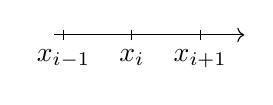
\begin{tikzpicture}[scale=.62]
\draw[->] (-.2,0)--(3.7,0);
\foreach \x/\lab in {0/$x_{i-1}$,1.4/$x_i$,2.8/$x_{i+1}$}{\draw (\x,.1)--(\x,-.1) node[below]{\lab};}
\end{tikzpicture}
\end{purplebox}
\end{column}
\end{columns}
\vspace{1mm}
\smallgray{Jika ruang data memungkinkan, formula pusat biasanya lebih disukai.}
\end{frame}

% ============ 11 HIGHER ACCURACY ============
\begin{frame}{Menaikkan akurasi: jangan berhenti di formula pertama}
\scriptsize
\begin{columns}[T,totalwidth=\textwidth]
\begin{column}{.50\textwidth}
\begin{bluebox}[Contoh beda maju orde lebih tinggi]
Dengan melibatkan titik $x_i$, $x_i+h$, dan $x_i+2h$,
\[
f'(x_i)\approx\frac{-3f_i+4f_{i+1}-f_{i+2}}{2h},
\]
\[
\text{galat }O(h^2).
\]
\end{bluebox}
\begin{orangebox}[Beda pusat orde lebih tinggi]
\[
f'(x_i)\approx\frac{f_{i-2}-8f_{i-1}+8f_{i+1}-f_{i+2}}{12h},
\]
\[
\text{galat }O(h^4).
\]
\end{orangebox}
\end{column}
\begin{column}{.46\textwidth}
\begin{greenbox}[Intuisi]
Semakin banyak titik digunakan, semakin banyak suku Taylor yang dapat dieliminasi. Akurasi meningkat, tetapi kebutuhan data juga bertambah.
\end{greenbox}
\begin{goldbox}[Perlu hati-hati]
Ukuran langkah yang terlalu kecil tidak selalu lebih baik karena pembulatan komputer ikut berperan.
\end{goldbox}
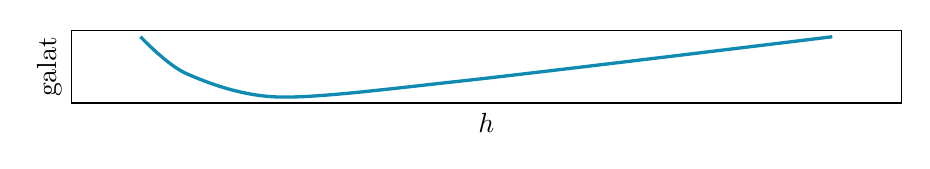
\begin{tikzpicture}
\begin{axis}[width=\linewidth,height=2.5cm,ymode=log,xlabel={$h$},ylabel={galat},grid=both,xtick=\empty,ytick=\empty]
\addplot[Teal,very thick,smooth] coordinates {(0.05,0.08) (.1,0.025) (.2,0.012) (.4,0.02) (.8,0.08)};
\end{axis}
\end{tikzpicture}
\end{column}
\end{columns}
\end{frame}

% ============ 12 NEWTON POLYNOMIAL ============
\begin{frame}{Polinom Newton: menghampiri fungsi dulu, lalu diturunkan}
\scriptsize
\begin{columns}[T,totalwidth=\textwidth]
\begin{column}{.52\textwidth}
\begin{bluebox}[Interpolasi polinom]
Dari titik data, bentuk polinom yang melewati titik-titik tersebut:
\[
p(t)=b_0+b_1(t-t_0)+b_2(t-t_0)(t-t_1)+\cdots.
\]
Turunan fungsi kemudian dihampiri dengan
\[
f'(t)\approx p'(t).
\]
\end{bluebox}
\begin{orangebox}[Koefisien awal]
\[
b_0=f(t_0),\qquad
b_1=\frac{f(t_1)-f(t_0)}{t_1-t_0}.
\]
\end{orangebox}
\end{column}
\begin{column}{.44\textwidth}
\begin{tikzpicture}
\begin{axis}[width=\linewidth,height=5.2cm,axis lines=middle,xmin=-.2,xmax=3.2,ymin=.2,ymax=3.5,xtick={0,1,2},xticklabels={$t_0$,$t_1$,$t_2$},ytick=\empty]
\addplot[only marks,mark=*,mark size=2.2pt,Orange] coordinates {(0,1.1) (1,1.8) (2,2.2)};
\addplot[domain=0:2.2,Teal,very thick,samples=100]{1.1+0.95*x-0.25*x*(x-1)};
\node[font=\scriptsize,anchor=west] at (axis cs:1.75,2.9) {$p(t)$};
\end{axis}
\end{tikzpicture}
\smallgray{Beda hingga dapat dipandang sebagai turunan dari polinom interpolasi lokal.}
\end{column}
\end{columns}
\end{frame}

% ============ 13 NEWTON TO FINITE DIFF ============
\begin{frame}{Dari Polinom Newton ke formula beda hingga}
\scriptsize
\begin{columns}[T,totalwidth=\textwidth]
\begin{column}{.50\textwidth}
\begin{bluebox}[Ambil tiga titik]
\[
t_0=x,
\qquad t_1=x+h,
\qquad t_2=x+2h.
\]
Polinom kuadratik:
\[
p(t)=b_0+b_1(t-t_0)+b_2(t-t_0)(t-t_1).
\]
Turunannya:
\[
p'(t)=b_1+b_2\{(t-t_0)+(t-t_1)\}.
\]
\end{bluebox}
\end{column}
\begin{column}{.46\textwidth}
\begin{orangebox}[Evaluasi di titik x]
Setelah $b_1$ dan $b_2$ disubstitusi,
\[
f'(x)\approx p'(x)
=\frac{-3f(x)+4f(x+h)-f(x+2h)}{2h}.
\]
\end{orangebox}
\begin{greenbox}[Latihan cepat]
Coba ulangi dengan $t_0=x$, $t_1=x-h$, $t_2=x-2h$. Formula apa yang muncul?
\end{greenbox}
\end{column}
\end{columns}
\end{frame}

% ============ 14 RICHARDSON ============
\begin{frame}{Ide ekstrapolasi Richardson}
\scriptsize
\begin{columns}[T,totalwidth=\textwidth]
\begin{column}{.50\textwidth}
\begin{bluebox}[Dua hampiran dengan galat terstruktur]
Misalkan suatu hampiran $D(h)$ memiliki bentuk
\[
D(h)=D^\ast+C h^p+O(h^{p+1}).
\]
Jika dihitung juga dengan langkah $h/2$:
\[
D(h/2)=D^\ast+C\left(\frac{h}{2}\right)^p+O(h^{p+1}).
\]
\end{bluebox}
\end{column}
\begin{column}{.46\textwidth}
\begin{orangebox}[Eliminasi suku galat utama]
\[
D_R=\frac{2^pD(h/2)-D(h)}{2^p-1}.
\]
Untuk beda pusat turunan pertama, biasanya $p=2$:
\[
D_R=\frac{4D(h/2)-D(h)}{3}.
\]
\end{orangebox}
\begin{greenbox}[Intuisi]
Kita tidak hanya memperkecil $h$, tetapi juga memakai pola galat untuk memperbaiki hasil.
\end{greenbox}
\end{column}
\end{columns}
\end{frame}

% ============ 15 RICHARDSON EXAMPLE ============
\begin{frame}{Contoh mini: Richardson pada beda pusat}
\scriptsize
\begin{bluebox}[Langkah kerja]
Pilih satu fungsi dan titik $x_i$. Hitung beda pusat dengan dua ukuran langkah:
\[
D(h)=\frac{f(x_i+h)-f(x_i-h)}{2h},
\]
\[
D(h/2)=\frac{f(x_i+h/2)-f(x_i-h/2)}{h}.
\]
Kemudian
\[
D_R=\frac{4D(h/2)-D(h)}{3}.
\]
\end{bluebox}
\begin{columns}[T,totalwidth=\textwidth]
\begin{column}{.48\textwidth}
\begin{orangebox}[Yang diamati]
\begin{itemize}\setlength\itemsep{2pt}
\item Apakah $D(h/2)$ selalu lebih dekat dari $D(h)$?
\item Apakah $D_R$ lebih baik dari keduanya?
\item Bagaimana pola galatnya?
\end{itemize}
\end{orangebox}
\end{column}
\begin{column}{.48\textwidth}
\begin{greenbox}[Grafik yang berguna]
\begin{itemize}\setlength\itemsep{2pt}
\item $h$ versus galat.
\item metode versus galat.
\item tabel $D(h),D(h/2),D_R$.
\end{itemize}
\end{greenbox}
\end{column}
\end{columns}
\end{frame}

% ============ 16 MATLAB ============
\begin{frame}[fragile]{Demo komputasi singkat}
\scriptsize
\begin{columns}[T,totalwidth=\textwidth]
\begin{column}{.56\textwidth}
\begin{bluebox}[Formula dalam kode]
\begin{verbatim}
f  = @(x) -0.1*x.^4 -0.15*x.^3 ...
          -0.5*x.^2 -0.25*x + 1.25;
df = @(x) -0.4*x.^3 -0.45*x.^2 -x -0.25;
xi = 0.5;
h  = 0.5;

Dmaju  = (f(xi+h)-f(xi))/h;
Dmund  = (f(xi)-f(xi-h))/h;
Dpusat = (f(xi+h)-f(xi-h))/(2*h);
DR     = (4*((f(xi+h/2)-f(xi-h/2))/h) - Dpusat)/3;
D      = [Dmaju Dmund Dpusat DR];
err    = abs(D-df(xi))/abs(df(xi));
bar(err)
\end{verbatim}
\end{bluebox}
\end{column}
\begin{column}{.40\textwidth}
\begin{orangebox}[Output yang diharapkan]
\begin{itemize}\setlength\itemsep{2pt}
\item Tabel hampiran.
\item Tabel galat relatif.
\item Grafik perbandingan galat.
\item Kesimpulan singkat: metode mana paling baik pada contoh ini?
\end{itemize}
\end{orangebox}
\begin{greenbox}[Catatan]
Gunakan 
\[
\frac{|D_{num}-D_{eksak}|}{\max(1,|D_{eksak}|)}
\]
agar tetap aman ketika nilai pembanding kecil.
\end{greenbox}
\end{column}
\end{columns}
\end{frame}

% ============ 17 LATIHAN ============
\begin{frame}{Latihan mandiri}
\scriptsize
\begin{orangebox}[Soal 1]
Diketahui
\[
f(x)=25x^3-6x^2+7x-88.
\]
Gunakan beda maju, beda mundur, dan beda pusat untuk menghampiri $f'(2)$ dengan $h=0.2$.
Bandingkan dengan turunan eksak.
\end{orangebox}
\begin{greenbox}[Soal 2]
Gunakan fungsi pada Soal 1. Hitung hampiran beda pusat dengan $h=0.2$ dan $h=0.1$, kemudian lakukan ekstrapolasi Richardson.
Tampilkan tabel dan grafik galat.
\end{greenbox}
\begin{purplebox}[Soal 3]
Turunkan formula beda pusat orde lebih tinggi
\[
f'(x_i)\approx\frac{f_{i-2}-8f_{i-1}+8f_{i+1}-f_{i+2}}{12h}.
\]
Petunjuk: tuliskan Taylor untuk $x_i\pm h$ dan $x_i\pm2h$, lalu eliminasi suku $f^{(3)}$.
\end{purplebox}
\end{frame}

% ============ 18 NEXT DISCUSSION ============
\begin{frame}{Bahan presentasi berikutnya}
\scriptsize
\begin{bluebox}[Bagian A: soal yang dibuat sendiri]
Pilih satu fungsi dan satu titik. Gunakan satu metode beda hingga, lalu perbaiki hasilnya dengan ekstrapolasi Richardson. Sajikan tabel, grafik galat, dan kesimpulan.
\end{bluebox}
\begin{orangebox}[Bagian B: satu problem dari artikel ilmiah]
Pilih satu artikel yang memakai turunan numerik, beda hingga, atau estimasi laju perubahan. Ikuti metode pada artikel, lalu gunakan ekstrapolasi Richardson sebagai pembanding jika memungkinkan.
\end{orangebox}
\begin{greenbox}[Yang dipresentasikan]
\begin{enumerate}\setlength\itemsep{2pt}
\item Fungsi/model/data yang dipakai.
\item Metode beda yang digunakan dan alasan pemilihannya.
\item Hasil sebelum dan sesudah ekstrapolasi.
\item Grafik galat atau grafik perbandingan hasil.
\item Apa yang berubah setelah hasil diperbaiki?
\end{enumerate}
\end{greenbox}
\end{frame}

\end{document}
